\label{cap:diseno-implementacion}

En este capítulo se indican los pasos seguidos a la hora de elaborar el diseño y la implementación de los algoritmos de los modelos de clasificación.
\\

\section{Variable objetivo y variables de entrada}
\label{sec:dis-variables}

La \gls{variable-objetivo} del modelo es la clase de accesibilidad, una variable ordinal que puede tomar como valores A, B y C, de mayor a menor accesibilidad.
\\

Existen cuatro variables objetivo, una por cada perfil de diversidad (funcional, sensorial y cognitivo) y una global, en el conjunto unificado de datos (tabla~\ref{tab:columnas-unificadas}): \texttt{clase\_total}, \texttt{clase\_funcional}, \texttt{clase\_sensorial} y \texttt{clase\_cognitiva}.
\\

En cuanto a las variables de entrada, se van a utilizar las 28 puntuaciones por dimensión, \texttt{puntuacion\_*\_*}, una por cada combinación de las siete dimensiones (pendiente, anchura, pavimento, cruces, señalización, iluminación y mobiliario) y las cuatro puntuaciones: la global y las de los tres perfiles de diversidad (funcional, sensorial y cognitivo). Por ejemplo, \texttt{puntuacion\_pendiente\_global} o \texttt{puntuacion\_cruces\_sensorial}.
\\

Quedan fuera las cuatro puntuaciones totales (\texttt{puntuacion\_total}, \texttt{puntuacion\_total\_funcional}, \texttt{puntuacion\_total\_sensorial} y \texttt{puntuacion\_total\_cognitiva}), por provocar \gls{fuga-informacion}: la clase se calcula directamente a partir de ellas.
\\

\sintesisdecision{
  \item \sintesisclave{Variables objetivo} \texttt{clase\_total}, \texttt{clase\_funcional}, \texttt{clase\_sensorial} y \texttt{clase\_cognitiva}.
  \item \sintesisclave{Variables de entrada} las 28 puntuaciones \texttt{puntuacion\_*\_*}, sin las cuatro puntuaciones totales.}

\section{División de los datos}
\label{sec:dis-division}

Se ha comprobado si los tramos de una misma calle son similares entre sí, así como los tramos de cada barrio. Al comparar la puntuación total de un tramo con la de otro tramo de su misma calle, la diferencia media es menor que con un tramo elegido al azar de la misma ciudad (0,104 frente a 0,130 en Albacete, y 0,144 frente a 0,160 en Algeciras). La relación es pequeña (en Algeciras, la diferencia entre ambas medias es de solo 0,016), por lo que la agrupación por calle se mantiene como precaución. La razón de fondo es metodológica (subsección~\ref{subsec:validacion-conclusiones}): evitar que tramos casi idénticos de una misma calle acaben en entrenamiento y en test.
\\

Se ha evaluado también la agrupación por barrio, pero se ha descartado. Los barrios tienen tamaños muy desiguales (entre 1 y 79 tramos por barrio en Algeciras) y los tramos de clase A se concentran en pocos de ellos (2 de los 27 barrios de Albacete y 11 de los 44 de Algeciras). Como consecuencia, al agrupar por barrio los 24 tramos de clase A de Albacete caen en un único pliegue de test, y en Algeciras hay un pliegue de test sin ninguno.
\\

Por lo tanto, la división de los datos \textbf{se agrupa por calle} (columna \texttt{nombre\_calle\_base}), de forma que todos los tramos de una calle quedan en el mismo conjunto (o bien de entrenamiento, o de test). Concuerda con la conclusión de la subsección~\ref{subsec:validacion-conclusiones} (figura~\ref{fig:split-misma-calle}).
\\

\begin{figure}[htbp]
  \centering
  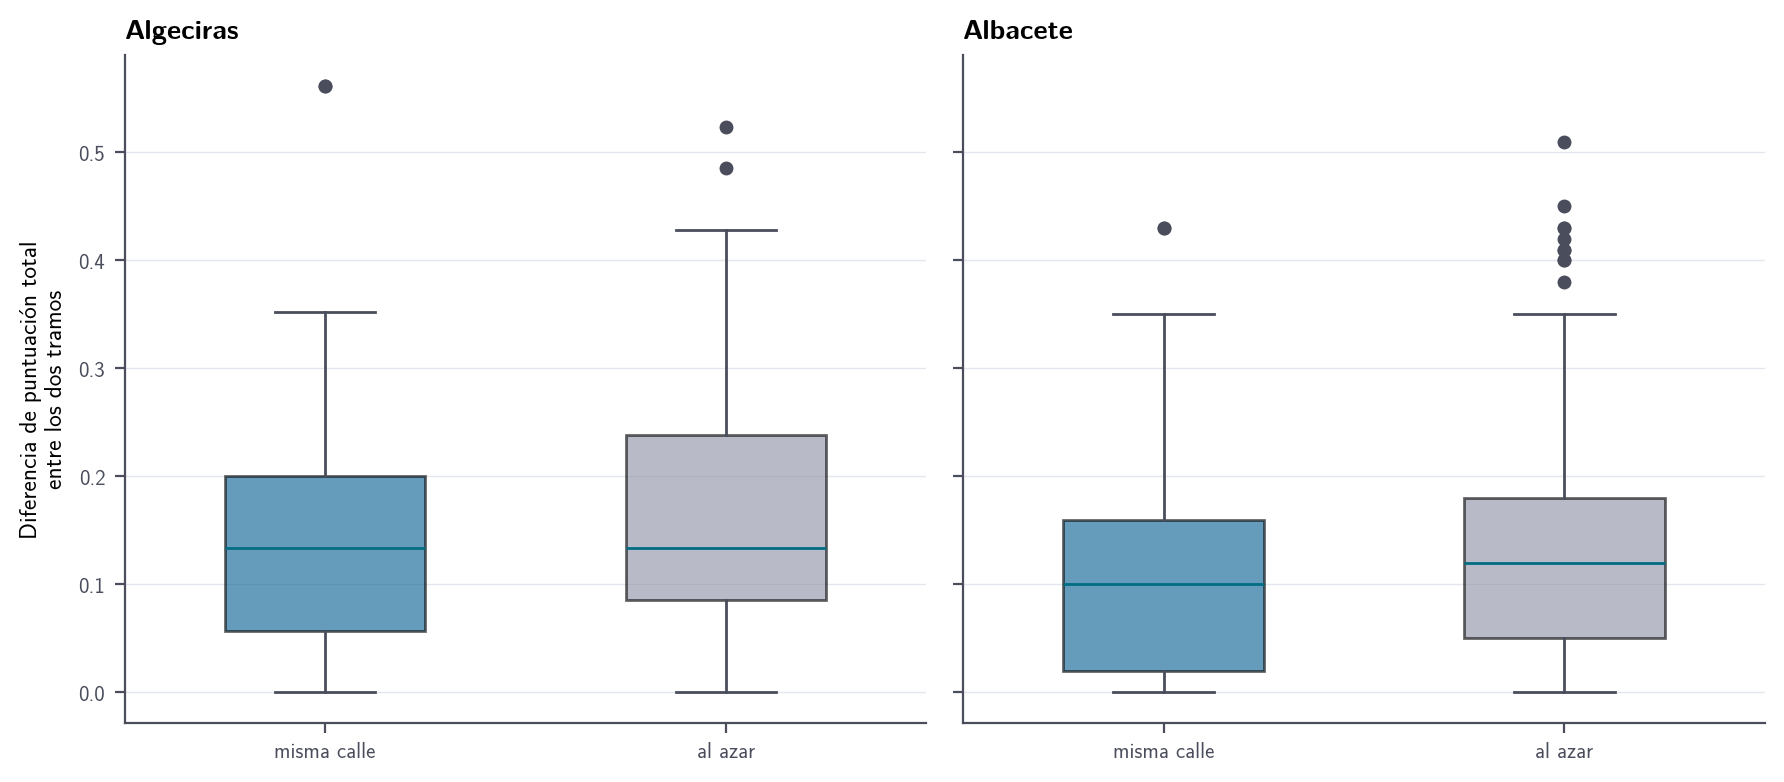
\includegraphics[width=0.8\linewidth]{capitulos/05-diseno-implementacion/figuras/diferencia_misma_calle_vs_azar.png}
  \caption{Diferencia de puntuación total entre un tramo y otro de su misma calle, o de un tramo al azar de la ciudad.}
  \label{fig:split-misma-calle}
  \fuente{Elaboración propia.}
\end{figure}

Para evaluar los modelos se va a utilizar \gls{validacion-cruzada}: el conjunto de datos se divide en varios subconjuntos disjuntos, denominados \glspl{pliegue} (\textit{folds}). En cada iteración, uno de los pliegues se reserva para test y los restantes se usan para entrenamiento, de forma que cada pliegue actúa como test una vez. Se han establecido 5 pliegues.
\\

El conjunto de datos es bastante desbalanceado, y la clase A es muy minoritaria (24 tramos en Albacete y 28 en Algeciras). Es necesario que los pliegues se hagan teniendo en cuenta esto, para evitar que existan algunos con muy pocos tramos de clase A (o ninguno), tanto en entrenamiento como en test.
\\

Como se busca tener pliegues con una proporción parecida de tramos de clase A, B y C a la del conjunto de datos completo, se ha decidido utilizar \texttt{StratifiedGroupKFold} de \textit{scikit-learn}. Permite realizar la agrupación por calle, y además reparte las clases de manera proporcional (\gls{estratificacion}), en base a la \texttt{clase\_total}. Se estratifica siempre con esta clase, también para los modelos de cada perfil de diversidad, para que todos los modelos usen los mismos pliegues y la comparación entre ellos sea justa. Se ha establecido una \gls{semilla} (\textit{seed}) fija con valor 42, para poder reproducir la división.
\\

La estratificación es aproximada, porque las calles no se pueden partir: con la agrupación por calle, algunos pliegues de test tienen solo 2 tramos de clase A (en ambas ciudades). Por ello, se informará de la variabilidad de las métricas entre pliegues, y no solo de su media.
\\

Se contemplan tres estrategias de división (tabla~\ref{tab:estrategias-division}). En la estrategia entre ciudades no hay pliegues, sino una única partición por sentido (de Albacete a Algeciras, y viceversa).

\begin{table}[htbp]
  \centering
  \caption{Estrategias de división de los datos.}
  \label{tab:estrategias-division}
  \small
  \begin{tabularx}{\textwidth}{>{\raggedright\arraybackslash}p{0.17\textwidth} >{\raggedright\arraybackslash}X >{\raggedright\arraybackslash}X >{\raggedright\arraybackslash}X}
    \toprule
    \cabeceratabla Estrategia & Entrenamiento & Test & Qué contrasta \\
    \midrule
    Dentro de cada ciudad & 4 pliegues de la misma ciudad (Albacete o Algeciras). & 1 pliegue de esa ciudad. & Rendimiento en una ciudad. \\
    Entre ciudades & Todos los tramos de una ciudad. & Todos los tramos de la otra ciudad (sin pliegues). & Transferibilidad entre ciudades (H4). \\
    Mezclada & 4 pliegues con las dos ciudades juntas. & 1 pliegue con las dos ciudades. & Rendimiento con ambas ciudades. \\
    \bottomrule
  \end{tabularx}
  \fuente{Elaboración propia.}
\end{table}

\sintesisdecision{
  \item \sintesisclave{Agrupación} por calle (\texttt{nombre\_calle\_base}), no por barrio.
  \item \sintesisclave{Validación} cruzada con \texttt{StratifiedGroupKFold}, 5 pliegues, estratificada con \texttt{clase\_total} y semilla 42.
  \item \sintesisclave{Estrategias} dentro de cada ciudad, entre ciudades y mezclada.}
